\begin{myproof}[of Proposition \ref{pro:scale_factor}] 
\label{proof:scale_factor}
\normalfont
In the following, we prove a more general statement: Let $\mathcal{Q}$ be a convex polygon, and let $\mathcal{P}$ be another convex polygon that entirely covers $\mathcal{Q}$. Then, for any two arbitrary points $s$ and $t$ outside of $\mathcal{P}$, we have
\begin{equation}
\label{statement}
\nonumber 
\left|  L_\mathcal{P}(s,t) \right |  \leq  \left|  L_\mathcal{Q}(s,t) \right |  +  p_\mathcal{P} - p_\mathcal{Q} (*)
\end{equation}
Figure \ref{fig:pro_1} illustrates the proof.
%\noindent \textbf{Proof (of Proposition \ref{lem:lemma1}).}\\
Let $Q_1, ..., Q_n$ denote the vertices of $\mathcal{Q}$, and let $P_1, ..., P_m$ denote the vertices of $\mathcal{P}$, which are ordered in the counterclockwise direction.
Let $s{ \{Q_u \sim Q_{u+k} \}}^{+}_\mathcal{Q} t$ denote the shortest path between $s$ and $t$ that bypasses $\mathcal{Q}$, and assume that this path stays on the right side of $\overrightarrow{st}$.
According to Proposition \ref{pro:shortest_path}, $Q_u$ and $Q_{u+k}$ must be view-limit vertices of $\mathcal{Q}$ with respect to $s$ and $t$, respectively.
%\begin{figure}[bt]
%	\centering
%	\includegraphics[width =0.35\columnwidth]{strategy_4.eps}
%	\vspace{-8pt}
%	\caption{Illustration of the proof of Theorem \ref{lem:strategy_4}.\label{fig:strategy_4}}
%\end{figure}
Let $P_v, .., P_{v+h}$ denote all vertices of $\mathcal{P}$ that are on the right side of $\overrightarrow{st}$; then, $L_\mathcal{P}(s,t) \leq s{ \{ P_v \sim P_{v+h} \} }^{+}_\mathcal{P}t$. 
Let $Q^{'}_{u}$ and $Q^{'}_{u+k}$ denote the intersections of $sQ_u$ and $tQ_{u+k}$ with $P_{v-1}P_v$ and $P_{v+h}P_{v+h+1}$, respectively. Then,  
\begin{footnotesize}
\begin{equation}
\label{eq:n_4_1}
L_\mathcal{P}(s,t)  \leq s{ \{ P_v \sim P_{v+h} \} }^{+}_\mathcal{P}t 
 \leq \left |sQ^{'}_{u} \right | + \left | { \{ Q^{'}_{u} \sim Q^{'}_{u+k}\} }^{+}_\mathcal{P} \right | + \left |Q^{'}_{u+k}t \right |  
\end{equation}
\end{footnotesize}
%\begin{equation}
%\begin{split}
%\label{eq:n_4_1}
%l_\mathcal{P}(s,t) & \leq s{ \{ P_v \sim P_{v+h} \} }_\mathcal{P}t \\
%& \leq \left |sQ^{'}_{u} \right | + \left | { \{ Q^{'}_{u} \sim Q^{'}_{u+k}\} }_\mathcal{P} \right | + \left |Q^{'}_{u+k}t \right |  
%\end{split}
%\end{equation}
It is obvious that
\begin{footnotesize}
\begin{equation}
\label{eq:n_4_2}
\left | Q_{u+k} Q^{'}_{u+k} \right | + \left | { \{ Q^{'}_{u+k} \sim Q^{'}_{u} \} }^{+}_\mathcal{P}\right | + \left | Q^{'}_{u}Q_u\right | \geq \left | {\{ Q_{u+k} \sim Q_u \}}^{+}_\mathcal{Q}\right |  
\end{equation}
\end{footnotesize}
Note that $p_\mathcal{P}= \left | { \{ Q^{'}_{u} \sim Q^{'}_{u+k} \} }^{+}_\mathcal{P}\right | +  \left | { \{ Q^{'}_{u+k} \sim Q^{'}_{u} \} }^{+}_\mathcal{P}\right | $.
Therefore, from (\ref{eq:n_4_2}), it can be deduced that
\begin{footnotesize}
\begin{equation}
\label{eq:n_4_3}
\left | { \{ Q^{'}_{u} \sim Q^{'}_{u+k} \} }^{+}_\mathcal{P}\right | \leq p_\mathcal{P} -  \left | {\{ Q_{u+k} \sim Q_u \}}^{+}_\mathcal{Q}\right |  
+ \left | Q_{u+k} Q^{'}_{u+k} \right | +  \left | Q^{'}_{u}Q_u\right | 
\end{equation}
\end{footnotesize}
%\begin{equation}
%\begin{split}
%\label{eq:n_4_3}
%\left | { \{ Q^{'}_{u} \sim Q^{'}_{u+k} \} }_\mathcal{P}\right | \leq p_\mathcal{P} &-  \left | {\{ Q_{u+k} \sim Q_u \}}_\mathcal{Q}\right |  \\
%&+ \left | Q_{u+k} Q^{'}_{u+k} \right | +  \left | Q^{'}_{u}Q_u\right | 
%\end{split}
%\end{equation}
Note that $p_\mathcal{Q}= \left | { \{ Q_{u} \sim Q_{u+k} \} }^{+}_\mathcal{Q}\right | +  \left | { \{ Q_{u+k} \sim Q_{u} \} }^{+}_\mathcal{Q}\right | $.\\
Therefore, (\ref{eq:n_4_3}) is equivalent to
\begin{equation}
\begin{split}
\label{eq:n_4_4}
\left | { \{ Q^{'}_{u} \sim Q^{'}_{u+k} \} }^{+}_\mathcal{P}\right | \leq p_\mathcal{P} - p_\mathcal{Q}  & +  \left | { \{ Q_{u} \sim Q_{u+k} \} }^{+}_\mathcal{Q}\right |  \\
& + \left | Q_{u+k} Q^{'}_{u+k} \right | +  \left | Q^{'}_{u}Q_u\right | 
\end{split}
\end{equation}
By adding (\ref{eq:n_4_1}) and (\ref{eq:n_4_4}), we obtain
\begin{equation}
\nonumber L_\mathcal{P}(s,t) \leq   L_\mathcal{Q}(s,t) + p_\mathcal{P} - p_\mathcal{Q}
\end{equation}
Thus, Statement (*) is proven. Proposition \ref{pro:scale_factor} can be directly deduced from Statement (\ref{statement}) as follows.
Because $\mathcal{F}$ is an image of $\mathcal{H}$ obtained through a homothetic transformation with a scale factor of $\xi$, $p_{\mathcal{F}} = (1-\xi)p_{\mathcal{H}}$.
Therefore, $L_\mathcal{F}(s,t) \leq  L_\mathcal{H}(s,t) + p_\mathcal{F} - p_\mathcal{H} = L_\mathcal{H}(s,t) + (\xi-1)p_\mathcal{H}$.
\end{myproof} 
\begin{figure}[hbt]
	\centering
	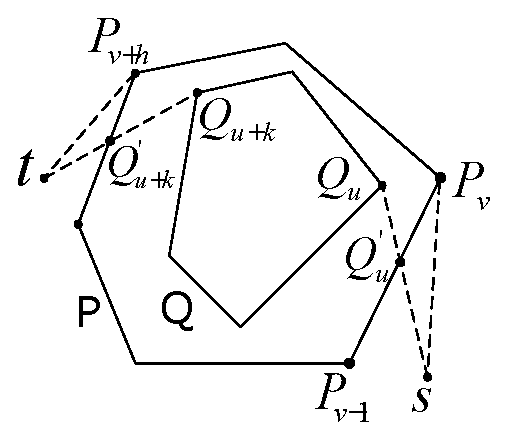
\includegraphics[width =0.35\columnwidth]{./appendix/proof_1.eps}
	\caption{Illustration of the proof of  Proposition \ref{pro:scale_factor}.\label{fig:pro_1}}
\end{figure}
